\documentclass[10pt]{article}
\usepackage[utf8]{inputenc}\usepackage[T1]{fontenc}
\usepackage[margin=1.45cm]{geometry}\usepackage{graphicx,booktabs,tabularx,xcolor,hyperref}
\graphicspath{{../../evidencia/figuras/}}
\definecolor{navy}{HTML}{184E77}\definecolor{teal}{HTML}{2A9D8F}\definecolor{soft}{HTML}{EDF5FB}
\hypersetup{colorlinks=true,linkcolor=navy,urlcolor=teal}\setlength{\parindent}{0pt}\setlength{\parskip}{4pt}
\newcommand{\kpi}[1]{\colorbox{soft}{\strut\textbf{#1}}}
\begin{document}
{\color{navy}\LARGE\bfseries Proyecto 1: Monitoreo transaccional}\\[-1mm]
{\large Detectar lo que el orden revela}\hfill Grupo 1 · Sección 30\\
\textbf{Wilson Alejandro Calderón Argueta (22018)} · \textbf{Pablo Daniel Barillas Moreno (22193)}\\
Universidad del Valle de Guatemala · Deep Learning y Sistemas Inteligentes · Kevin Recinos
\vspace{2mm}\hrule\vspace{2mm}

\section*{Resumen ejecutivo}
Se evaluó si el orden de las transacciones añade valor frente al sistema agregado del Banco del Altiplano. Sobre 590,540 transacciones reales anonimizadas de IEEE-CIS (20,663 fraudes; 3.499\%), se compararon A: gradient boosting sobre agregados, B: GRU sobre ocho eventos y C: fusión GRU--agregados. La selección se realizó con validación cronológica y prueba se abrió una vez. El candidato fue \textbf{A}. La permutación solo cambió AUC-PR en 0.002; no se atribuye una ventaja material al orden. Conservar A como candidato y no migrar aún a secuencias. El costo usa Q4,200 por FN y Q180 por FP; la extrapolación mensual es un escenario, no una cifra contable.

\section*{1. Integridad de datos y protocolo temporal}
El origen es la competencia IEEE-CIS Fraud Detection de Kaggle, aportada por Vesta Corporation. Las transacciones cubren 182 días. La entidad se aproxima con \texttt{card1+card2+card3+card5+addr1}: permite historial, pero no garantiza identidad perfecta. Cada objetivo usa la transacción actual y hasta siete antecedentes; no usa futuro.

\begin{center}\small
\begin{tabular}{lrr}\toprule Partición & n & Fraude \\\midrule
Entrenamiento poblacional & 413,378 & 3.517\% \\
Validación & 88,581 & 3.434\% \\
Prueba final & 88,581 & 3.480\% \\\bottomrule
\end{tabular}\end{center}
Los primeros 70\% del tiempo entrenan, 15\% validan y 15\% prueban. Normalización, vocabularios, parada, arquitectura y umbrales se ajustan sin prueba. El submuestreo computacional ocurre solo dentro de entrenamiento y conserva todos los positivos; ambos modelos usan la misma muestra.
\begin{center}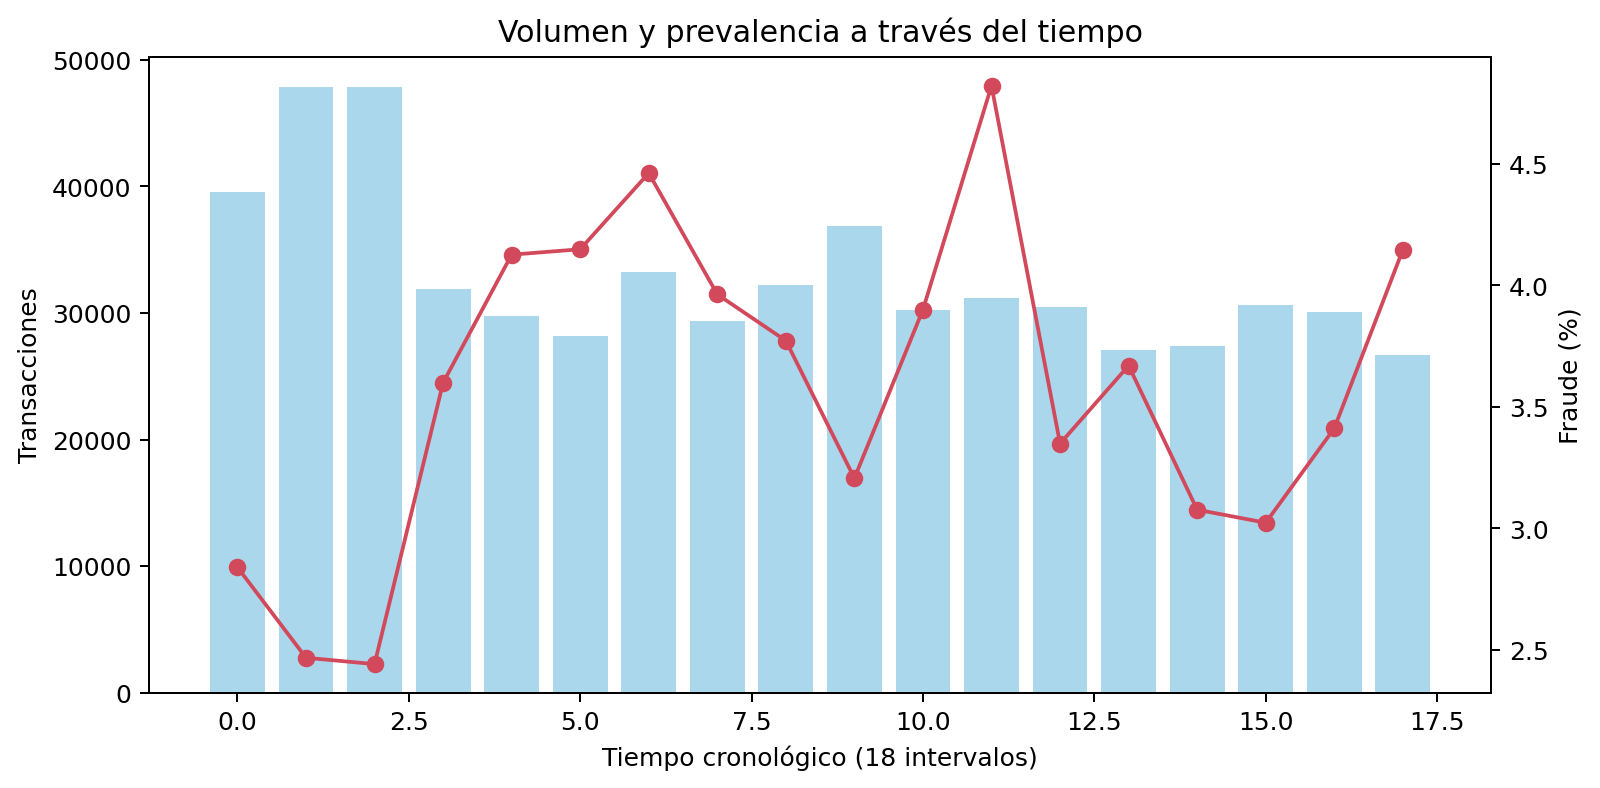
\includegraphics[width=.83\linewidth]{01_integridad_temporal.png}\end{center}

\section*{2. Núcleo A--B y apuesta C}
\textbf{A} resume nivel, dispersión, extremos, recencia y diversidad, y usa HistGradientBoosting. \textbf{B} codifica diez variables numéricas y seis categóricas por evento mediante embeddings y GRU(32). Ambos generan riesgo continuo. \textbf{C} concatena el estado final de B con agregados estandarizados. La hipótesis previa exigió que C aumentara AUC-PR al menos 0.01 y redujera costo al menos 5\% frente a B en validación. El cambio observado fue -0.001 y 0.3\%; la apuesta fue \textbf{no útil según el criterio previo}.

\section*{3. Comparación común}
\begin{center}\small\begin{tabular}{lrrrrr}\toprule Modelo & AUC-PR & Prec. & Recall & F1 & Costo test \\\midrule
A & 0.429 & 0.134 & 0.722 & 0.226 & Q6,193,620 \\
B & 0.412 & 0.154 & 0.649 & 0.248 & Q6,525,960 \\
C & 0.392 & 0.136 & 0.671 & 0.226 & Q6,618,900 \\
\bottomrule\end{tabular}\end{center}
AUC-PR es principal por el desbalance; precisión, recall y F1 se reportan en el umbral económico propio, fijado con validación. Exactitud no se usa para decidir.
\begin{center}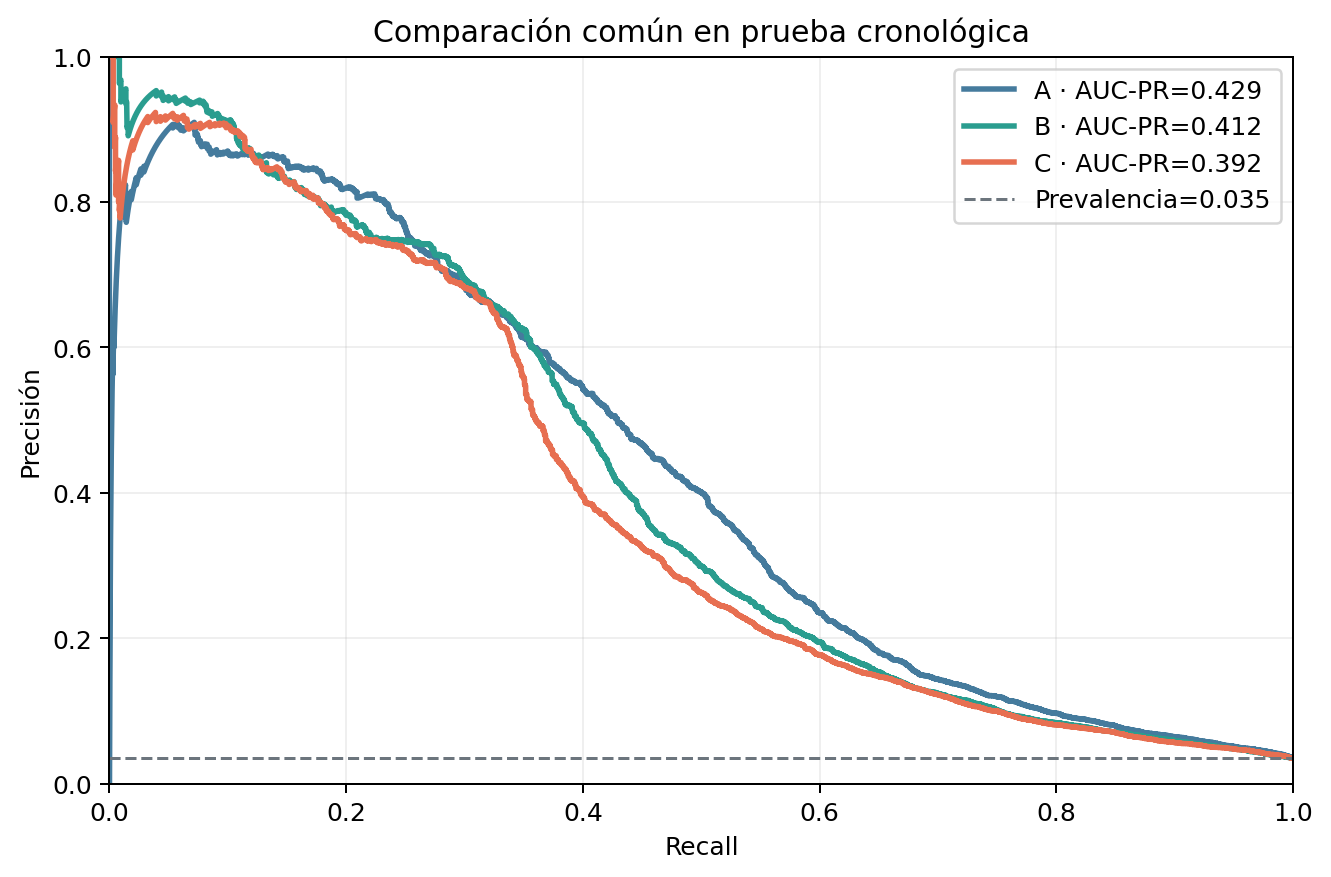
\includegraphics[width=.80\linewidth]{02_curvas_precision_recall.png}\end{center}

\section*{4. Intentos de refutar el valor del orden}
Se permutó cinco veces solo la historia, manteniendo la transacción objetivo al final y todos los eventos intactos. B obtuvo AUC-PR 0.412 original y 0.410$\pm$0.001 permutada. La permutación solo cambió AUC-PR en 0.002; no se atribuye una ventaja material al orden. La segunda prueba recortó el historial a tres eventos y produjo AUC-PR 0.411. Estas pruebas miden dependencia predictiva, no causalidad ni identidad bancaria perfecta.
\begin{center}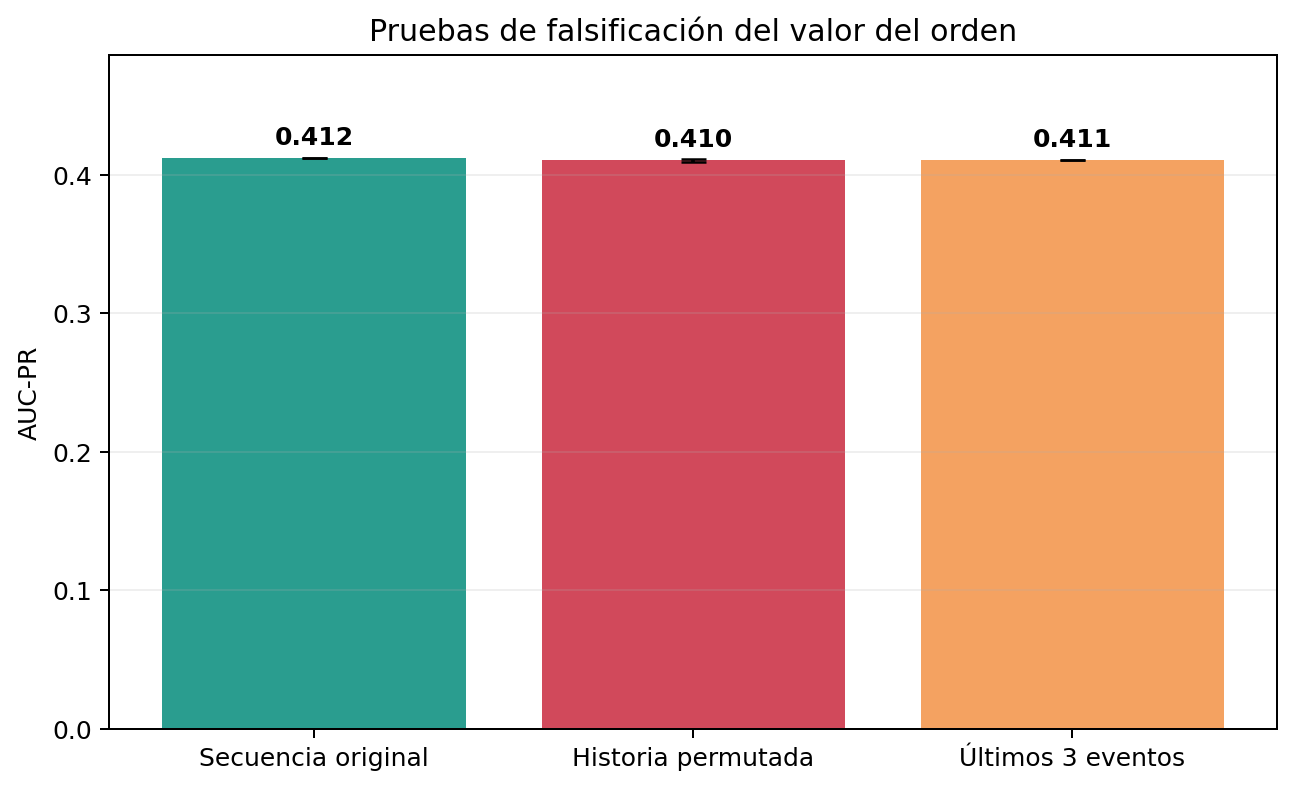
\includegraphics[width=.75\linewidth]{03_falsificaciones_orden.png}\end{center}

\section*{5. Umbral, costo y decisión}
Se minimizó en validación $C(\tau)=4200FN(\tau)+180FP(\tau)$. Para A, el costo de prueba es Q6,193,620, equivalente a Q6,992,041 por 100 mil decisiones. Con 1.4 millones de tarjetas y 12 transacciones mensuales, el escenario escalado es Q1,174,662,919. Frente a A, B perdería Q63,030,582 al mes y C perdería Q80,657,297 al mes. La prevalencia y el volumen reales deben reemplazar estos supuestos antes de una decisión financiera.
\begin{center}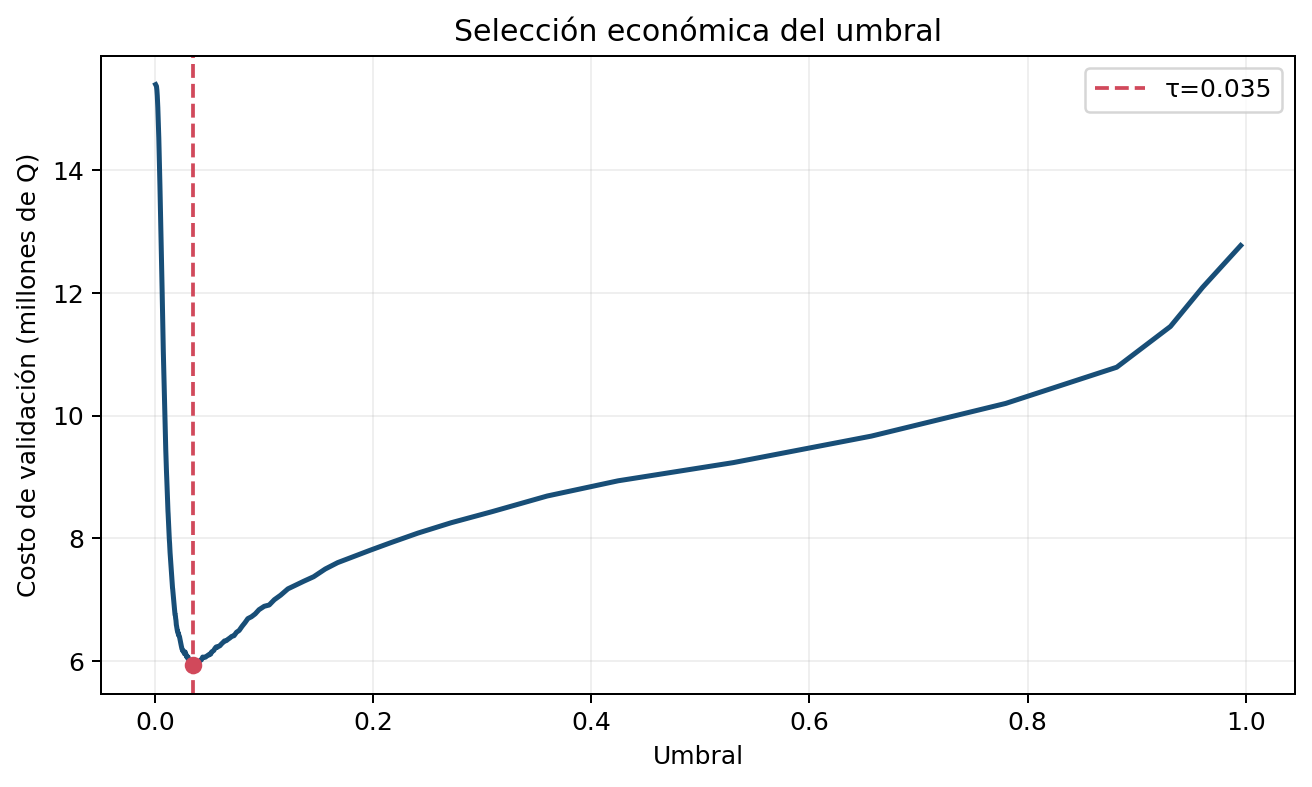
\includegraphics[width=.75\linewidth]{04_curva_costo_umbral.png}\end{center}

\section*{6. Recomendación, errores y límites}
\textbf{Conservar A como candidato y no migrar aún a secuencias.} El puntaje debe priorizar revisión, no bloquear automáticamente. Un patrón concreto del candidato es que 222 de 858 falsos negativos (25.9\%) son ProductCD=W con monto en (68.5, 117.0]; es una concentración descriptiva, no causal. Cambiaríamos la recomendación si una clave de tarjeta confiable elimina el efecto, si una cohorte posterior revierte AUC-PR/costo o si revisión no absorbe alertas. Límites: identidad aproximada, anonimización, 182 días, una ventana, costos transferidos, ausencia de latencia, calibración externa, deriva, equidad y piloto humano.

\section*{Matriz de evidencias}
\scriptsize\begin{tabularx}{\linewidth}{p{2.4cm}p{2.5cm}X X}\toprule Evidencia & Ubicación & Conclusión & Limitación \\\midrule
Integridad & Fig. 1, Tabla 1 & 70/15/15 cronológico; ajustes train-only & Entidad aproximada \\
Comparación A--B & Fig. 2, Tabla 2 & Mismo horizonte y AUC-PR & Historial de 8 eventos \\
Valor del orden & Fig. 3 & Permutación repetida y recorte & Dependencia no implica causalidad \\
Apuesta C & Sección 2 & Criterio fijado antes del test & Mayor complejidad \\
Economía & Fig. 4 & Umbral minimiza costo suministrado & Volumen/prevalencia asumidos \\
Recomendación & Sección 6 & Decisión condicionada & Falta piloto productivo \\\bottomrule
\end{tabularx}

\section*{Referencias}
\footnotesize
Cho, K., et al. (2014). \textit{Learning phrase representations using RNN encoder-decoder}. \url{https://arxiv.org/abs/1406.1078}.\\
Fisher, A., Rudin, C., \& Dominici, F. (2019). All models are wrong, but many are useful. \textit{JMLR, 20}(177), 1--81.\\
IEEE Computational Intelligence Society. (2019). \textit{IEEE-CIS Fraud Detection} [Data set]. Kaggle.\\
Saito, T., \& Rehmsmeier, M. (2015). The precision-recall plot is more informative than ROC. \textit{PLOS ONE, 10}(3), e0118432.\\
Scikit-learn Developers. (s. f.). \textit{Common pitfalls and recommended practices}. \url{https://scikit-learn.org/stable/common_pitfalls.html}.
\end{document}
